\documentclass[aspectratio=169,11pt]{beamer}
\usepackage[T1]{fontenc}
\usepackage{tikz}
\usetikzlibrary{arrows.meta,positioning}

\usetheme{metropolis}
\usepackage[sfdefault]{FiraSans}
\definecolor{unitnred}{HTML}{B10B25}
\definecolor{slideblue}{HTML}{2B5FA3}
\definecolor{slidegray}{HTML}{8A8F98}
\setbeamercolor{progress bar}{fg=unitnred}
\setbeamercolor{alerted text}{fg=unitnred}
\setbeamerfont{frametitle}{size=\large}
\setbeamertemplate{navigation symbols}{}
\hyphenpenalty=10000
\exhyphenpenalty=10000
\tolerance=3000
\emergencystretch=3em

\tikzset{flowbox/.style={draw, rounded corners=2pt, inner sep=6pt,
  align=center, minimum height=15mm},
  flowarrow/.style={-{Stealth[length=3mm]}, thick},
  flow/.style={font=\small, node distance=7mm}}

\setbeamerfont{title}{size=\LARGE}
\setbeamerfont{subtitle}{size=\normalsize}

\title{Privacy Preserving LLM Orchestration for Enterprise Workflows}
\subtitle{Substituting Real Employee Data Before It Reaches the AI Model}
\author{Ettore Miglioranza\\[1.5mm]{\small Supervisor: Prof.\ Daniele Miorandi\\[0.5mm]Co Supervisor: Massimo Turri \textmd{(Saidea S.r.l.)}}}
\institute{University of Trento}
\date{15 September 2026}
\titlegraphic{%
  \begin{tikzpicture}[remember picture, overlay]
    \node[anchor=north east, xshift=-5mm, yshift=-4mm] at (current page.north east)
      {
\includegraphics[height=0.9cm]{figures/unitn_logo.png}};
  \end{tikzpicture}}

\begin{document}

% ============================================================
% Slide 1: Title
% ============================================================
\begin{frame}[plain]
  \titlepage
\end{frame}

% ============================================================
% Slide 2: Problem
% ============================================================
\begin{frame}{Data protection requirements constrain what an AI assistant may access}
  \begin{columns}[c]
    \column{0.42\textwidth}
      {\Huge\bfseries\color{unitnred} 40\%}\\[1mm]
      {\small Of professionals identify data privacy as the leading ethical concern with generative AI, up from 25\% the previous year}\\[2.5mm]
      {\footnotesize\color{slidegray} Deloitte, \emph{State of Ethics and Trust in Technology}, $\sim$1{,}848 respondents, Sept.\ 2024}
    \column{0.54\textwidth}
      {\small A representative request to the system:}\\[2mm]
      {\small\ttfamily "Trova i colleghi di \textcolor{unitnred}{\bfseries Giulia Conti}"}\\[3mm]
      {\footnotesize\color{slidegray} This name constitutes personal data under the GDPR (Art.\ 4(1)). Transmission to an external AI model discloses it outside the company boundary}
  \end{columns}
\end{frame}

% ============================================================
% Slide 3: The gap and the research question
% ============================================================
\begin{frame}{Existing architectures require a choice between model capability and data exposure}
  \small
  \begin{columns}[t]
    \column{0.48\textwidth}
      {\color{slidegray}\footnotesize ASSUMED BY EXISTING SYSTEMS}\\[1mm]
      The model is trusted directly with raw data\\[2mm]
      Alternatively, the model is denied access to the data entirely
    \column{0.48\textwidth}
      {\color{unitnred}\footnotesize REQUIRED BY THIS DEPLOYMENT}\\[1mm]
      The model's full reasoning capability\\[2mm]
      No exposure of real names, addresses, or phone numbers to the model
  \end{columns}
  \vspace{4mm}\pause
  \begin{quote}\itshape\footnotesize\raggedright
    Can an AI model be granted operational authority over sensitive company
    workflows without direct access to the underlying data, in a way that holds
    under measurement rather than under assumption?
  \end{quote}
  \vspace{2mm}
  {\footnotesize\color{slidegray} Plain MCP passes raw text to the model unmodified; one-way redaction discards data with no way back (Anthropic 2024, OpenAI 2026)}
\end{frame}

% ============================================================
% Slide 4: Why four separate services
% ============================================================
\begin{frame}{The architecture separates identity resolution from decision making across four services}
  \small
  Antares AI, a deployed workforce management product\\[3mm]
  \begin{itemize}
    \setlength{\itemsep}{0.3cm}
    \item A local service identifies the sensitive parts of the request
    \item A separate store holds only the mapping between each real value and its placeholder
    \item The AI model receives a placeholder for every sensitive part the detector identifies
    \item Real values and the corresponding decision are combined only within the company server, for the duration of the action
  \end{itemize}
\end{frame}

% ============================================================
% Slide 5: Approach / mechanism
% ============================================================
\begin{frame}{The model decides which action to take; the server holds the real values}
  \centering
  \vfill
  \resizebox{0.75\linewidth}{!}{%
  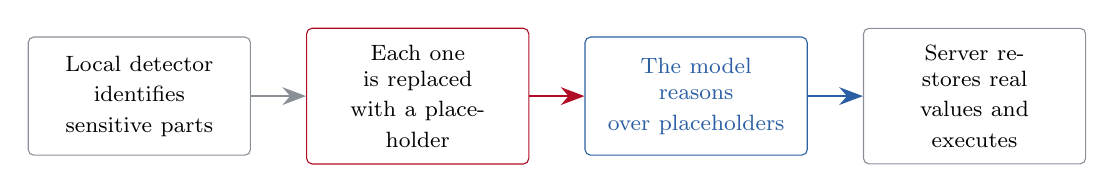
\begin{tikzpicture}[flow]
    \node[flowbox, draw=slidegray, text width=2.4cm] (a) {\footnotesize Local detector\\identifies sensitive parts};
    \node[flowbox, right=of a, draw=unitnred, text width=2.4cm] (b) {\footnotesize Each one is replaced\\with a placeholder};
    \node[flowbox, right=of b, draw=slideblue, text=slideblue, text width=2.4cm] (c) {\footnotesize The model reasons\\over placeholders};
    \node[flowbox, right=of c, draw=slidegray, text width=2.4cm] (d) {\footnotesize Server restores real\\values and executes};
    \draw[flowarrow, slidegray] (a) -- (b);
    \draw[flowarrow, unitnred] (b) -- (c);
    \draw[flowarrow, slideblue] (c) -- (d);
  \end{tikzpicture}}\\[2mm]
  \vfill
\end{frame}

% ============================================================
% Slide 6: Start to finish example
% ============================================================
\begin{frame}{A worked example: one request traced through the pipeline}
  \centering
  \vspace{1mm}
  \resizebox{0.98\linewidth}{!}{%
  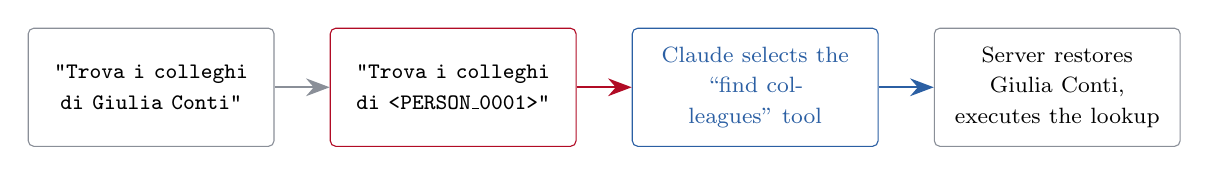
\begin{tikzpicture}[flow]
    \node[flowbox, draw=slidegray, text width=2.7cm] (a) {\footnotesize\ttfamily "Trova i colleghi\\di Giulia Conti"};
    \node[flowbox, right=of a, draw=unitnred, text width=2.7cm] (b) {\footnotesize\ttfamily "Trova i colleghi\\di <PERSON\_0001>"};
    \node[flowbox, right=of b, draw=slideblue, text=slideblue, text width=2.7cm] (c) {\footnotesize Claude selects the\\``find colleagues'' tool};
    \node[flowbox, right=of c, draw=slidegray, text width=2.7cm] (d) {\footnotesize Server restores\\Giulia Conti, executes the lookup};
    \draw[flowarrow, slidegray] (a) -- (b);
    \draw[flowarrow, unitnred] (b) -- (c);
    \draw[flowarrow, slideblue] (c) -- (d);
  \end{tikzpicture}}\\[6mm]
  {\small In this request, the text shown at stage two is the entire input the model receives}\\[1mm]
  {\footnotesize\color{slidegray} The response returned to the user contains the real names of Giulia's colleagues, restored only after the model has selected the action to perform}
\end{frame}

% ============================================================
% Slide 7: The role of MCP
% ============================================================
\begin{frame}{MCP standardises how the model reaches company tools}
  \small
  \vspace{2mm}
  \textbf{What it is}: MCP, the Model Context Protocol, is an open standard that lets an AI model reach outside services, like the one that just found Giulia's colleagues, in a common, predictable way\\[4mm]
  \textbf{Why it was chosen}: it separates the tool itself from the model, so the integration is not tied to one AI provider\\[4mm]
  \textbf{Without it}: each tool would need its own custom, model specific integration, rebuilt again for every different AI model
\end{frame}

% ============================================================
% Slide 8: The instrument
% ============================================================
\begin{frame}{Results are measured on the deployed system, not a synthetic benchmark}
  \small
  \begin{columns}[t]
    \column{0.5\textwidth}
      {\color{slidegray}\footnotesize SYSTEM UNDER TEST}\\[1mm]
      Antares AI, a deployed workforce management product\\[2mm]
      Italian language requests, personnel data by construction
    \column{0.5\textwidth}
      {\color{unitnred}\footnotesize VALIDATION METHOD}\\[1mm]
      Detection, exposure, and tool selection are measured separately, each on its own set of test requests\\[2mm]
      Evaluated against the product's own mock backend, not a separate research harness
  \end{columns}
\end{frame}

% ============================================================
% Slide 9: Result 1, detection
% ============================================================
\begin{frame}{What the detector catches is measured, not assumed}
  \centering
  \vspace{4mm}
  {\Huge\bfseries\color{slideblue} 91.5\%}\\[2mm]
  {\small Of the real names, places, and numbers in 50 manually verified test requests were correctly identified and replaced}\\[3mm]
  {\small\color{slidegray} Measuring what the detector misses requires test requests where every real entity has been labelled by hand first}\\[3mm]
  {\footnotesize\color{slidegray} Measured against 82 manually labelled examples. The remaining errors are concentrated in date ranges and email addresses}
\end{frame}

% ============================================================
% Slide 10: Result 2, leak audit
% ============================================================
\begin{frame}{The audit found limited, explained exposure}
  \centering
  \vspace{3mm}
  {\Huge\bfseries\color{unitnred} 2 / 50}\\[2mm]
  {\small Test requests in which a real name reached the AI model}\\[3mm]
  {\small\color{slidegray} The audit reuses the detection requests, scanning the exact text sent to the model for real values it should not contain}\\[3mm]
  {\footnotesize\color{slidegray} Both cases correspond to a detection error identified above; no leakage was observed through any other mechanism in these tests}
\end{frame}

% ============================================================
% Slide 11: Result 3, routing consistency
% ============================================================
\begin{frame}{Tool selection is consistent across repeated trials}
  \centering
  \vspace{4mm}
  {\Huge\bfseries\color{slideblue} 95.2\%}\\[2mm]
  {\small Correct company tool selected, in 100 of 105 repeated trials}\\[3mm]
  {\small\color{slidegray} Each request maps onto one expected tool}\\[3mm]
  {\footnotesize\color{slidegray} Each request was submitted five separate times; language model outputs are not guaranteed to be repeatable}
\end{frame}

% ============================================================
% Slide 12: What limits it
% ============================================================
\begin{frame}{Two limitations bound the scope of the privacy protection}
  \small
  \vspace{4mm}
  \textbf{The protection is contingent on server side trust}; placeholder mappings do not expire, and logs are stored without encryption\\[6mm]
  \textbf{No adversarial evaluation has been conducted}; the structural defence has not been tested against deliberate attack
\end{frame}

% ============================================================
% Slide 13: What this thesis adds
% ============================================================
\begin{frame}{Originality lies in the pipeline and its evaluation, not in its components}
  \small
  \vspace{2mm}
  \textbf{The integration pipeline}: detection, placeholder substitution, routing, and controlled restoration of data prior to action, designed and implemented for this deployment\\[4mm]
  \textbf{The evaluation methodology}: an independently implemented reference system, a leak audit on the exact text sent to the model, and a repeated trial routing evaluation, evaluating not just whether data is protected but whether the action executed is correct\\[4mm]
  The name detection model, the underlying AI model, and the MCP standard itself are adopted without modification and are not original contributions of this work\\[4mm]
  {\footnotesize\color{slidegray} The closest prior work evaluates privacy or reversibility, not the correctness of the action executed (Hou et al.\ 2025, Albanese et al.\ 2026)}
\end{frame}

% ============================================================
% Slide 14: Thank you
% ============================================================
\begin{frame}[plain]
  \centering
  \vspace{1.5cm}
  {\Large\bfseries Thank you}\\[4mm]
  {\normalsize Questions?}\\[1cm]
  {\small Ettore Miglioranza \\ \texttt{ettore.miglioranza@studenti.unitn.it}}
\end{frame}

% =========================================================
% Backup slides
% =========================================================
\begin{frame}[plain]
  \centering
  \vspace{2cm}
  {\Large\bfseries Backup}
\end{frame}

% ============================================================
% Backup A: Architecture components
% ============================================================
\begin{frame}{Backup: four cooperating services}
  \small
  \begin{itemize}
    \setlength{\itemsep}{0.25cm}
    \item \textbf{MCP Client} builds the raw prompt, calls the detection service, then hands off to the AI model with a context id, and receives no further real data after that first call.
    \item \textbf{Anonymisation API} runs detection and placeholder substitution, and restores real values on request from the server side only.
    \item \textbf{Detection service} is a stateless, off the shelf multilingual name, place, and number detector; it has no knowledge of placeholders or where they are stored.
    \item \textbf{MCP Server / JobTools} receives the AI model's tool call, restores the real values, and executes company logic, kept only on the server.
  \end{itemize}
\end{frame}

% ============================================================
% Backup B: Two conditions this design depends on
% ============================================================
\begin{frame}{Backup: two conditions this design depends on}
  \centering
  \vspace{4mm}
  \textbf{Detection recall is an empirical quantity}: measured directly against test prompts, not assumed to be complete\\[4mm]
  \textbf{Downstream execution must be deterministic and auditable}: ordinary server code, not another model inference
\end{frame}

% ============================================================
% Backup C: Methodology detail
% ============================================================
\begin{frame}{Backup: how each number was produced}
  \scriptsize
  \begin{itemize}
    \setlength{\itemsep}{0.2cm}
    \item \textbf{Detection:} 50 hand built Italian prompts, 82 labelled spans, coverage vs.\ strict span and label scoring.
    \item \textbf{Correctness:} Differential testing against an independent reference implementation, zero shared code with the system under test.
    \item \textbf{Leak audit:} The exact payload sent to the AI model, reconstructed client side, scanned for 39 known real values across 50 prompts.
    \item \textbf{Routing:} 21 prompts $\times$ 5 repetitions = 105 trials at temperature 1.0, checked by diffing timestamped log files.
  \end{itemize}
\end{frame}

% ============================================================
% Backup D: Correctness against an independent reference
% ============================================================
\begin{frame}{Backup: correctness against an independent reference}
  \centering
  \vspace{4mm}
  {\Huge\bfseries\color{slideblue} 12/12}\\[2mm]
  {\small Test requests matched an independently built reference implementation}\\[6mm]
  {\footnotesize\color{slidegray} Execution at this stage is deterministic: identical inputs produce identical outputs under the same server code, conventional and auditable rather than a further model inference}
\end{frame}

% ============================================================
% Backup E: Full limitations
% ============================================================
\begin{frame}{Backup: the complete limitations list}
  \scriptsize
  \begin{itemize}
    \setlength{\itemsep}{0.16cm}
    \item Placeholder mappings never expire and are read, not removed, on each restore, a real, unresolved tradeoff between reliability and data minimisation.
    \item Local logs are unencrypted, with no access control or retention policy.
    \item The connection between the AI model and the company server has no login step; any client that can reach it is accepted.
    \item A caller identity check exists but is designed to fail open rather than block access.
    \item No adversarial test set was built; the structural defence has not been attacked on purpose.
    \item Validation ran against a mock backend; one rarer workflow branch (finding a substitute during an absence) never fired within the test window.
    \item The routing check used 21 hand built prompts; consistency held on this fixed set, not on arbitrary phrasing.
  \end{itemize}
\end{frame}

\end{document}
